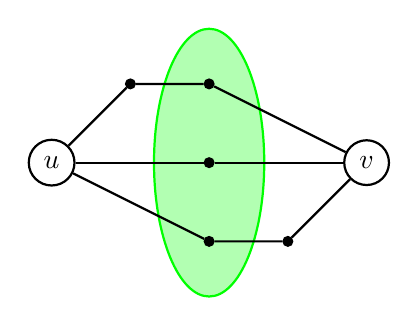
\begin{tikzpicture}[
  dot/.style = {
    shape = circle,
    fill = black,
    minimum size = 4pt,
    inner sep = 0pt,
    outer sep = 0pt,
  },
  point/.style = {
    circle,
    draw = black
  },
  every path/.style = {
    thick
  }
] 
  \draw[draw = green, fill = green!30] (2, 0) ellipse (0.7cm and 1.7cm);
  \node[point] (u) at (0, 0) {\(u\)};
  \node[dot] (p) at (1, 1) {};

  \node[dot] (x) at (2, 1) {};
  \node[dot] (mid) at (2, 0) {};
  \node[dot] (y) at (2, -1) {};

  \node[dot] (q) at (3, -1) {};
  \node[point] (v) at (4, 0) {\(v\)};

  \draw (u) -- (mid) -- (v);
  \draw (u) -- (p) -- (x) -- (v);
  \draw (u) -- (y) -- (q) -- (v);
\end{tikzpicture}
